

\tikzset{every picture/.style={line width=0.75pt}} %set default line width to 0.75pt        

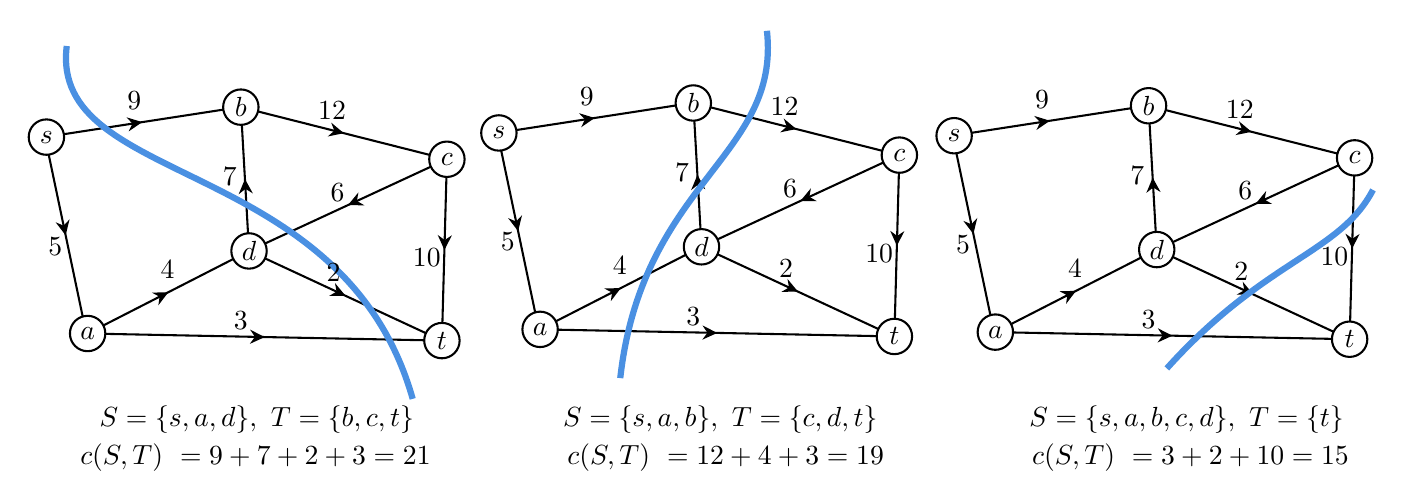
\begin{tikzpicture}[x=0.5pt,y=0.5pt,yscale=-1,xscale=1]
%uncomment if require: \path (0,338); %set diagram left start at 0, and has height of 338

%Straight Lines [id:da3853598268579197] 
\draw    (28.79,82.83) -- (169.31,61.18) ;
\draw [shift={(99.05,72)}, rotate = 531.24] [fill={rgb, 255:red, 0; green, 0; blue, 0 }  ][line width=0.08]  [draw opacity=0] (10.72,-5.15) -- (0,0) -- (10.72,5.15) -- (7.12,0) -- cycle    ;
%Straight Lines [id:da6958538828947681] 
\draw    (28.79,82.83) -- (58.58,224.77) ;
\draw [shift={(43.69,153.8)}, rotate = 258.15] [fill={rgb, 255:red, 0; green, 0; blue, 0 }  ][line width=0.08]  [draw opacity=0] (10.72,-5.15) -- (0,0) -- (10.72,5.15) -- (7.12,0) -- cycle    ;
%Straight Lines [id:da2980592918523626] 
\draw    (59.58,224.77) -- (315.62,229.9) ;
\draw [shift={(187.6,227.34)}, rotate = 181.15] [fill={rgb, 255:red, 0; green, 0; blue, 0 }  ][line width=0.08]  [draw opacity=0] (10.72,-5.15) -- (0,0) -- (10.72,5.15) -- (7.12,0) -- cycle    ;
%Straight Lines [id:da14604600957867897] 
\draw    (176.22,165.11) -- (315.62,229.9) ;
\draw [shift={(245.92,197.5)}, rotate = 204.92000000000002] [fill={rgb, 255:red, 0; green, 0; blue, 0 }  ][line width=0.08]  [draw opacity=0] (10.72,-5.15) -- (0,0) -- (10.72,5.15) -- (7.12,0) -- cycle    ;
%Straight Lines [id:da8640956582518242] 
\draw    (170.31,61.18) -- (176.22,165.11) ;
\draw [shift={(173.27,113.14)}, rotate = 86.75] [fill={rgb, 255:red, 0; green, 0; blue, 0 }  ][line width=0.08]  [draw opacity=0] (10.72,-5.15) -- (0,0) -- (10.72,5.15) -- (7.12,0) -- cycle    ;
%Straight Lines [id:da285469110869773] 
\draw    (170.31,61.18) -- (319.22,98.84) ;
\draw [shift={(244.76,80.01)}, rotate = 194.2] [fill={rgb, 255:red, 0; green, 0; blue, 0 }  ][line width=0.08]  [draw opacity=0] (10.72,-5.15) -- (0,0) -- (10.72,5.15) -- (7.12,0) -- cycle    ;
%Straight Lines [id:da8162300663234149] 
\draw    (319.22,98.84) -- (315.62,229.9) ;
\draw [shift={(317.42,164.37)}, rotate = 271.57] [fill={rgb, 255:red, 0; green, 0; blue, 0 }  ][line width=0.08]  [draw opacity=0] (10.72,-5.15) -- (0,0) -- (10.72,5.15) -- (7.12,0) -- cycle    ;
%Straight Lines [id:da5085854502811855] 
\draw    (319.22,98.84) -- (176.22,165.11) ;
\draw [shift={(247.72,131.98)}, rotate = 335.13] [fill={rgb, 255:red, 0; green, 0; blue, 0 }  ][line width=0.08]  [draw opacity=0] (10.72,-5.15) -- (0,0) -- (10.72,5.15) -- (7.12,0) -- cycle    ;
%Straight Lines [id:da4064365628912957] 
\draw    (176.22,165.11) -- (59.58,224.77) ;
\draw [shift={(117.9,194.94)}, rotate = 152.91] [fill={rgb, 255:red, 0; green, 0; blue, 0 }  ][line width=0.08]  [draw opacity=0] (10.72,-5.15) -- (0,0) -- (10.72,5.15) -- (7.12,0) -- cycle    ;
%Shape: Ellipse [id:dp651117123053256] 
\draw  [fill={rgb, 255:red, 255; green, 255; blue, 255 }  ,fill opacity=1 ] (17,82.83) .. controls (17,75.77) and (22.73,70.04) .. (29.79,70.04) .. controls (36.86,70.04) and (42.58,75.77) .. (42.58,82.83) .. controls (42.58,89.9) and (36.86,95.62) .. (29.79,95.62) .. controls (22.73,95.62) and (17,89.9) .. (17,82.83) -- cycle ;
%Shape: Ellipse [id:dp7399561756845123] 
\draw  [fill={rgb, 255:red, 255; green, 255; blue, 255 }  ,fill opacity=1 ] (157.52,61.18) .. controls (157.52,54.11) and (163.25,48.39) .. (170.31,48.39) .. controls (177.38,48.39) and (183.1,54.11) .. (183.1,61.18) .. controls (183.1,68.24) and (177.38,73.97) .. (170.31,73.97) .. controls (163.25,73.97) and (157.52,68.24) .. (157.52,61.18) -- cycle ;
%Shape: Ellipse [id:dp8268258265249401] 
\draw  [fill={rgb, 255:red, 255; green, 255; blue, 255 }  ,fill opacity=1 ] (306.43,98.84) .. controls (306.43,91.78) and (312.15,86.05) .. (319.22,86.05) .. controls (326.28,86.05) and (332.01,91.78) .. (332.01,98.84) .. controls (332.01,105.9) and (326.28,111.63) .. (319.22,111.63) .. controls (312.15,111.63) and (306.43,105.9) .. (306.43,98.84) -- cycle ;
%Shape: Ellipse [id:dp5421818862330341] 
\draw  [fill={rgb, 255:red, 255; green, 255; blue, 255 }  ,fill opacity=1 ] (163.43,165.11) .. controls (163.43,158.05) and (169.15,152.32) .. (176.22,152.32) .. controls (183.28,152.32) and (189.01,158.05) .. (189.01,165.11) .. controls (189.01,172.18) and (183.28,177.9) .. (176.22,177.9) .. controls (169.15,177.9) and (163.43,172.18) .. (163.43,165.11) -- cycle ;
%Shape: Ellipse [id:dp45600813719389455] 
\draw  [fill={rgb, 255:red, 255; green, 255; blue, 255 }  ,fill opacity=1 ] (46.79,224.77) .. controls (46.79,217.71) and (52.52,211.98) .. (59.58,211.98) .. controls (66.64,211.98) and (72.37,217.71) .. (72.37,224.77) .. controls (72.37,231.84) and (66.64,237.56) .. (59.58,237.56) .. controls (52.52,237.56) and (46.79,231.84) .. (46.79,224.77) -- cycle ;
%Shape: Ellipse [id:dp031187496945339066] 
\draw  [fill={rgb, 255:red, 255; green, 255; blue, 255 }  ,fill opacity=1 ] (302.83,229.9) .. controls (302.83,222.83) and (308.56,217.11) .. (315.62,217.11) .. controls (322.69,217.11) and (328.41,222.83) .. (328.41,229.9) .. controls (328.41,236.96) and (322.69,242.69) .. (315.62,242.69) .. controls (308.56,242.69) and (302.83,236.96) .. (302.83,229.9) -- cycle ;
%Straight Lines [id:da7435046067409884] 
\draw    (355.79,79.83) -- (496.31,58.18) ;
\draw [shift={(426.05,69)}, rotate = 531.24] [fill={rgb, 255:red, 0; green, 0; blue, 0 }  ][line width=0.08]  [draw opacity=0] (10.72,-5.15) -- (0,0) -- (10.72,5.15) -- (7.12,0) -- cycle    ;
%Straight Lines [id:da8387107518837462] 
\draw    (355.79,79.83) -- (385.58,221.77) ;
\draw [shift={(370.69,150.8)}, rotate = 258.15] [fill={rgb, 255:red, 0; green, 0; blue, 0 }  ][line width=0.08]  [draw opacity=0] (10.72,-5.15) -- (0,0) -- (10.72,5.15) -- (7.12,0) -- cycle    ;
%Straight Lines [id:da3219489964495771] 
\draw    (386.58,221.77) -- (642.62,226.9) ;
\draw [shift={(514.6,224.34)}, rotate = 181.15] [fill={rgb, 255:red, 0; green, 0; blue, 0 }  ][line width=0.08]  [draw opacity=0] (10.72,-5.15) -- (0,0) -- (10.72,5.15) -- (7.12,0) -- cycle    ;
%Straight Lines [id:da7100151765093478] 
\draw    (503.22,162.11) -- (642.62,226.9) ;
\draw [shift={(572.92,194.5)}, rotate = 204.92000000000002] [fill={rgb, 255:red, 0; green, 0; blue, 0 }  ][line width=0.08]  [draw opacity=0] (10.72,-5.15) -- (0,0) -- (10.72,5.15) -- (7.12,0) -- cycle    ;
%Straight Lines [id:da4338060480266903] 
\draw    (497.31,58.18) -- (503.22,162.11) ;
\draw [shift={(500.27,110.14)}, rotate = 86.75] [fill={rgb, 255:red, 0; green, 0; blue, 0 }  ][line width=0.08]  [draw opacity=0] (10.72,-5.15) -- (0,0) -- (10.72,5.15) -- (7.12,0) -- cycle    ;
%Straight Lines [id:da7182225488033221] 
\draw    (497.31,58.18) -- (646.22,95.84) ;
\draw [shift={(571.76,77.01)}, rotate = 194.2] [fill={rgb, 255:red, 0; green, 0; blue, 0 }  ][line width=0.08]  [draw opacity=0] (10.72,-5.15) -- (0,0) -- (10.72,5.15) -- (7.12,0) -- cycle    ;
%Straight Lines [id:da5940568426447731] 
\draw    (646.22,95.84) -- (642.62,226.9) ;
\draw [shift={(644.42,161.37)}, rotate = 271.57] [fill={rgb, 255:red, 0; green, 0; blue, 0 }  ][line width=0.08]  [draw opacity=0] (10.72,-5.15) -- (0,0) -- (10.72,5.15) -- (7.12,0) -- cycle    ;
%Straight Lines [id:da6584403815712339] 
\draw    (646.22,95.84) -- (503.22,162.11) ;
\draw [shift={(574.72,128.98)}, rotate = 335.13] [fill={rgb, 255:red, 0; green, 0; blue, 0 }  ][line width=0.08]  [draw opacity=0] (10.72,-5.15) -- (0,0) -- (10.72,5.15) -- (7.12,0) -- cycle    ;
%Straight Lines [id:da04611791534207066] 
\draw    (503.22,162.11) -- (386.58,221.77) ;
\draw [shift={(444.9,191.94)}, rotate = 152.91] [fill={rgb, 255:red, 0; green, 0; blue, 0 }  ][line width=0.08]  [draw opacity=0] (10.72,-5.15) -- (0,0) -- (10.72,5.15) -- (7.12,0) -- cycle    ;
%Shape: Ellipse [id:dp8684805017046724] 
\draw  [fill={rgb, 255:red, 255; green, 255; blue, 255 }  ,fill opacity=1 ] (344,79.83) .. controls (344,72.77) and (349.73,67.04) .. (356.79,67.04) .. controls (363.86,67.04) and (369.58,72.77) .. (369.58,79.83) .. controls (369.58,86.9) and (363.86,92.62) .. (356.79,92.62) .. controls (349.73,92.62) and (344,86.9) .. (344,79.83) -- cycle ;
%Shape: Ellipse [id:dp26598537007129874] 
\draw  [fill={rgb, 255:red, 255; green, 255; blue, 255 }  ,fill opacity=1 ] (484.52,58.18) .. controls (484.52,51.11) and (490.25,45.39) .. (497.31,45.39) .. controls (504.38,45.39) and (510.1,51.11) .. (510.1,58.18) .. controls (510.1,65.24) and (504.38,70.97) .. (497.31,70.97) .. controls (490.25,70.97) and (484.52,65.24) .. (484.52,58.18) -- cycle ;
%Shape: Ellipse [id:dp8446989445980774] 
\draw  [fill={rgb, 255:red, 255; green, 255; blue, 255 }  ,fill opacity=1 ] (633.43,95.84) .. controls (633.43,88.78) and (639.15,83.05) .. (646.22,83.05) .. controls (653.28,83.05) and (659.01,88.78) .. (659.01,95.84) .. controls (659.01,102.9) and (653.28,108.63) .. (646.22,108.63) .. controls (639.15,108.63) and (633.43,102.9) .. (633.43,95.84) -- cycle ;
%Shape: Ellipse [id:dp5784359228600563] 
\draw  [fill={rgb, 255:red, 255; green, 255; blue, 255 }  ,fill opacity=1 ] (490.43,162.11) .. controls (490.43,155.05) and (496.15,149.32) .. (503.22,149.32) .. controls (510.28,149.32) and (516.01,155.05) .. (516.01,162.11) .. controls (516.01,169.18) and (510.28,174.9) .. (503.22,174.9) .. controls (496.15,174.9) and (490.43,169.18) .. (490.43,162.11) -- cycle ;
%Shape: Ellipse [id:dp971944601404772] 
\draw  [fill={rgb, 255:red, 255; green, 255; blue, 255 }  ,fill opacity=1 ] (373.79,221.77) .. controls (373.79,214.71) and (379.52,208.98) .. (386.58,208.98) .. controls (393.64,208.98) and (399.37,214.71) .. (399.37,221.77) .. controls (399.37,228.84) and (393.64,234.56) .. (386.58,234.56) .. controls (379.52,234.56) and (373.79,228.84) .. (373.79,221.77) -- cycle ;
%Shape: Ellipse [id:dp1835030596812679] 
\draw  [fill={rgb, 255:red, 255; green, 255; blue, 255 }  ,fill opacity=1 ] (629.83,226.9) .. controls (629.83,219.83) and (635.56,214.11) .. (642.62,214.11) .. controls (649.69,214.11) and (655.41,219.83) .. (655.41,226.9) .. controls (655.41,233.96) and (649.69,239.69) .. (642.62,239.69) .. controls (635.56,239.69) and (629.83,233.96) .. (629.83,226.9) -- cycle ;
%Curve Lines [id:da2649473788057739] 
\draw [color={rgb, 255:red, 74; green, 144; blue, 226 }  ,draw opacity=1 ][line width=2.25]    (44.5,17) .. controls (31.5,120) and (244.5,95) .. (294.5,272) ;
%Curve Lines [id:da16888389279841676] 
\draw [color={rgb, 255:red, 74; green, 144; blue, 226 }  ,draw opacity=1 ][line width=2.25]    (550.5,6) .. controls (560.5,97) and (460.5,115) .. (444.5,257) ;
%Straight Lines [id:da23959710765930176] 
\draw    (684.79,81.83) -- (825.31,60.18) ;
\draw [shift={(755.05,71)}, rotate = 531.24] [fill={rgb, 255:red, 0; green, 0; blue, 0 }  ][line width=0.08]  [draw opacity=0] (10.72,-5.15) -- (0,0) -- (10.72,5.15) -- (7.12,0) -- cycle    ;
%Straight Lines [id:da6431206981927323] 
\draw    (684.79,81.83) -- (714.58,223.77) ;
\draw [shift={(699.69,152.8)}, rotate = 258.15] [fill={rgb, 255:red, 0; green, 0; blue, 0 }  ][line width=0.08]  [draw opacity=0] (10.72,-5.15) -- (0,0) -- (10.72,5.15) -- (7.12,0) -- cycle    ;
%Straight Lines [id:da5596554414836099] 
\draw    (715.58,223.77) -- (971.62,228.9) ;
\draw [shift={(843.6,226.34)}, rotate = 181.15] [fill={rgb, 255:red, 0; green, 0; blue, 0 }  ][line width=0.08]  [draw opacity=0] (10.72,-5.15) -- (0,0) -- (10.72,5.15) -- (7.12,0) -- cycle    ;
%Straight Lines [id:da8160720971935526] 
\draw    (832.22,164.11) -- (971.62,228.9) ;
\draw [shift={(901.92,196.5)}, rotate = 204.92000000000002] [fill={rgb, 255:red, 0; green, 0; blue, 0 }  ][line width=0.08]  [draw opacity=0] (10.72,-5.15) -- (0,0) -- (10.72,5.15) -- (7.12,0) -- cycle    ;
%Straight Lines [id:da3877819200248832] 
\draw    (826.31,60.18) -- (832.22,164.11) ;
\draw [shift={(829.27,112.14)}, rotate = 86.75] [fill={rgb, 255:red, 0; green, 0; blue, 0 }  ][line width=0.08]  [draw opacity=0] (10.72,-5.15) -- (0,0) -- (10.72,5.15) -- (7.12,0) -- cycle    ;
%Straight Lines [id:da057104792707504015] 
\draw    (826.31,60.18) -- (975.22,97.84) ;
\draw [shift={(900.76,79.01)}, rotate = 194.2] [fill={rgb, 255:red, 0; green, 0; blue, 0 }  ][line width=0.08]  [draw opacity=0] (10.72,-5.15) -- (0,0) -- (10.72,5.15) -- (7.12,0) -- cycle    ;
%Straight Lines [id:da14831136034761006] 
\draw    (975.22,97.84) -- (971.62,228.9) ;
\draw [shift={(973.42,163.37)}, rotate = 271.57] [fill={rgb, 255:red, 0; green, 0; blue, 0 }  ][line width=0.08]  [draw opacity=0] (10.72,-5.15) -- (0,0) -- (10.72,5.15) -- (7.12,0) -- cycle    ;
%Straight Lines [id:da2506057291921263] 
\draw    (975.22,97.84) -- (832.22,164.11) ;
\draw [shift={(903.72,130.98)}, rotate = 335.13] [fill={rgb, 255:red, 0; green, 0; blue, 0 }  ][line width=0.08]  [draw opacity=0] (10.72,-5.15) -- (0,0) -- (10.72,5.15) -- (7.12,0) -- cycle    ;
%Straight Lines [id:da7375159787579277] 
\draw    (832.22,164.11) -- (715.58,223.77) ;
\draw [shift={(773.9,193.94)}, rotate = 152.91] [fill={rgb, 255:red, 0; green, 0; blue, 0 }  ][line width=0.08]  [draw opacity=0] (10.72,-5.15) -- (0,0) -- (10.72,5.15) -- (7.12,0) -- cycle    ;
%Shape: Ellipse [id:dp7941672492891375] 
\draw  [fill={rgb, 255:red, 255; green, 255; blue, 255 }  ,fill opacity=1 ] (673,81.83) .. controls (673,74.77) and (678.73,69.04) .. (685.79,69.04) .. controls (692.86,69.04) and (698.58,74.77) .. (698.58,81.83) .. controls (698.58,88.9) and (692.86,94.62) .. (685.79,94.62) .. controls (678.73,94.62) and (673,88.9) .. (673,81.83) -- cycle ;
%Shape: Ellipse [id:dp3757660056746118] 
\draw  [fill={rgb, 255:red, 255; green, 255; blue, 255 }  ,fill opacity=1 ] (813.52,60.18) .. controls (813.52,53.11) and (819.25,47.39) .. (826.31,47.39) .. controls (833.38,47.39) and (839.1,53.11) .. (839.1,60.18) .. controls (839.1,67.24) and (833.38,72.97) .. (826.31,72.97) .. controls (819.25,72.97) and (813.52,67.24) .. (813.52,60.18) -- cycle ;
%Shape: Ellipse [id:dp9316219699822907] 
\draw  [fill={rgb, 255:red, 255; green, 255; blue, 255 }  ,fill opacity=1 ] (962.43,97.84) .. controls (962.43,90.78) and (968.15,85.05) .. (975.22,85.05) .. controls (982.28,85.05) and (988.01,90.78) .. (988.01,97.84) .. controls (988.01,104.9) and (982.28,110.63) .. (975.22,110.63) .. controls (968.15,110.63) and (962.43,104.9) .. (962.43,97.84) -- cycle ;
%Shape: Ellipse [id:dp2713572714021609] 
\draw  [fill={rgb, 255:red, 255; green, 255; blue, 255 }  ,fill opacity=1 ] (819.43,164.11) .. controls (819.43,157.05) and (825.15,151.32) .. (832.22,151.32) .. controls (839.28,151.32) and (845.01,157.05) .. (845.01,164.11) .. controls (845.01,171.18) and (839.28,176.9) .. (832.22,176.9) .. controls (825.15,176.9) and (819.43,171.18) .. (819.43,164.11) -- cycle ;
%Shape: Ellipse [id:dp8303944409855877] 
\draw  [fill={rgb, 255:red, 255; green, 255; blue, 255 }  ,fill opacity=1 ] (702.79,223.77) .. controls (702.79,216.71) and (708.52,210.98) .. (715.58,210.98) .. controls (722.64,210.98) and (728.37,216.71) .. (728.37,223.77) .. controls (728.37,230.84) and (722.64,236.56) .. (715.58,236.56) .. controls (708.52,236.56) and (702.79,230.84) .. (702.79,223.77) -- cycle ;
%Shape: Ellipse [id:dp3672414292204079] 
\draw  [fill={rgb, 255:red, 255; green, 255; blue, 255 }  ,fill opacity=1 ] (958.83,228.9) .. controls (958.83,221.83) and (964.56,216.11) .. (971.62,216.11) .. controls (978.69,216.11) and (984.41,221.83) .. (984.41,228.9) .. controls (984.41,235.96) and (978.69,241.69) .. (971.62,241.69) .. controls (964.56,241.69) and (958.83,235.96) .. (958.83,228.9) -- cycle ;
%Curve Lines [id:da42045420214553086] 
\draw [color={rgb, 255:red, 74; green, 144; blue, 226 }  ,draw opacity=1 ][line width=2.25]    (988.5,121) .. controls (964.5,167) and (910.5,171) .. (839.5,250) ;

% Text Node
\draw (29.79,82.83) node   [align=left] {$\displaystyle s$};
% Text Node
\draw (170.31,61.18) node   [align=left] {$\displaystyle b$};
% Text Node
\draw (319.22,98.84) node   [align=left] {$\displaystyle c$};
% Text Node
\draw (176.22,165.11) node   [align=left] {$\displaystyle d$};
% Text Node
\draw (59.58,224.77) node   [align=left] {$\displaystyle a$};
% Text Node
\draw (315.62,229.9) node   [align=left] {$\displaystyle t$};
% Text Node
\draw (29,153) node [anchor=north west][inner sep=0.75pt]   [align=left] {$\displaystyle 5$};
% Text Node
\draw (110,170) node [anchor=north west][inner sep=0.75pt]   [align=left] {$\displaystyle 4$};
% Text Node
\draw (86,48) node [anchor=north west][inner sep=0.75pt]   [align=left] {$\displaystyle 9$};
% Text Node
\draw (233,114) node [anchor=north west][inner sep=0.75pt]   [align=left] {$\displaystyle 6$};
% Text Node
\draw (155,103) node [anchor=north west][inner sep=0.75pt]   [align=left] {$\displaystyle 7$};
% Text Node
\draw (230,172) node [anchor=north west][inner sep=0.75pt]   [align=left] {$\displaystyle 2$};
% Text Node
\draw (292.42,161.37) node [anchor=north west][inner sep=0.75pt]   [align=left] {$\displaystyle 10$};
% Text Node
\draw (224,55) node [anchor=north west][inner sep=0.75pt]   [align=left] {$\displaystyle 12$};
% Text Node
\draw (163,207) node [anchor=north west][inner sep=0.75pt]   [align=left] {$\displaystyle 3$};
% Text Node
\draw (356.79,79.83) node   [align=left] {$\displaystyle s$};
% Text Node
\draw (497.31,58.18) node   [align=left] {$\displaystyle b$};
% Text Node
\draw (646.22,95.84) node   [align=left] {$\displaystyle c$};
% Text Node
\draw (503.22,162.11) node   [align=left] {$\displaystyle d$};
% Text Node
\draw (386.58,221.77) node   [align=left] {$\displaystyle a$};
% Text Node
\draw (642.62,226.9) node   [align=left] {$\displaystyle t$};
% Text Node
\draw (356,150) node [anchor=north west][inner sep=0.75pt]   [align=left] {$\displaystyle 5$};
% Text Node
\draw (437,167) node [anchor=north west][inner sep=0.75pt]   [align=left] {$\displaystyle 4$};
% Text Node
\draw (413,45) node [anchor=north west][inner sep=0.75pt]   [align=left] {$\displaystyle 9$};
% Text Node
\draw (560,111) node [anchor=north west][inner sep=0.75pt]   [align=left] {$\displaystyle 6$};
% Text Node
\draw (482,100) node [anchor=north west][inner sep=0.75pt]   [align=left] {$\displaystyle 7$};
% Text Node
\draw (557,169) node [anchor=north west][inner sep=0.75pt]   [align=left] {$\displaystyle 2$};
% Text Node
\draw (619.42,158.37) node [anchor=north west][inner sep=0.75pt]   [align=left] {$\displaystyle 10$};
% Text Node
\draw (551,52) node [anchor=north west][inner sep=0.75pt]   [align=left] {$\displaystyle 12$};
% Text Node
\draw (490,204) node [anchor=north west][inner sep=0.75pt]   [align=left] {$\displaystyle 3$};
% Text Node
\draw (52,302.5) node [anchor=north west][inner sep=0.75pt]   [align=left] {$\displaystyle c( S,T) \ =9+7+2+3=21$};
% Text Node
\draw (404,302.5) node [anchor=north west][inner sep=0.75pt]   [align=left] {$\displaystyle c( S,T) \ =12+4+3=19$};
% Text Node
\draw (685.79,81.83) node   [align=left] {$\displaystyle s$};
% Text Node
\draw (826.31,60.18) node   [align=left] {$\displaystyle b$};
% Text Node
\draw (975.22,97.84) node   [align=left] {$\displaystyle c$};
% Text Node
\draw (832.22,164.11) node   [align=left] {$\displaystyle d$};
% Text Node
\draw (715.58,223.77) node   [align=left] {$\displaystyle a$};
% Text Node
\draw (971.62,228.9) node   [align=left] {$\displaystyle t$};
% Text Node
\draw (685,152) node [anchor=north west][inner sep=0.75pt]   [align=left] {$\displaystyle 5$};
% Text Node
\draw (766,169) node [anchor=north west][inner sep=0.75pt]   [align=left] {$\displaystyle 4$};
% Text Node
\draw (742,47) node [anchor=north west][inner sep=0.75pt]   [align=left] {$\displaystyle 9$};
% Text Node
\draw (889,113) node [anchor=north west][inner sep=0.75pt]   [align=left] {$\displaystyle 6$};
% Text Node
\draw (811,102) node [anchor=north west][inner sep=0.75pt]   [align=left] {$\displaystyle 7$};
% Text Node
\draw (886,171) node [anchor=north west][inner sep=0.75pt]   [align=left] {$\displaystyle 2$};
% Text Node
\draw (948.42,160.37) node [anchor=north west][inner sep=0.75pt]   [align=left] {$\displaystyle 10$};
% Text Node
\draw (880,54) node [anchor=north west][inner sep=0.75pt]   [align=left] {$\displaystyle 12$};
% Text Node
\draw (819,206) node [anchor=north west][inner sep=0.75pt]   [align=left] {$\displaystyle 3$};
% Text Node
\draw (740,302.5) node [anchor=north west][inner sep=0.75pt]   [align=left] {$\displaystyle c( S,T) \ =3+2+10=15$};
% Text Node
\draw (66,274.5) node [anchor=north west][inner sep=0.75pt]   [align=left] {$\displaystyle S=\{s,a,d\} ,\ T=\{b,c,t\}$};
% Text Node
\draw (401,274.5) node [anchor=north west][inner sep=0.75pt]   [align=left] {$\displaystyle S=\{s,a,b\} ,\ T=\{c,d,t\}$};
% Text Node
\draw (738,274.5) node [anchor=north west][inner sep=0.75pt]   [align=left] {$\displaystyle S=\{s,a,b,c,d\} ,\ T=\{t\}$};


\end{tikzpicture}

